\documentclass[10pt,a4paper]{article}

%%%%%%%%%%%%%%%%% CJK 中文版面控制  %%%%%%%%%%%%%%%%%%%%%%%%%%%%%%
\usepackage{xeCJK} % CTEX-CJK 中文支持                            %
\usepackage{CJKutf8} % Texlive 中文支持                          %
\usepackage{CJKnumb} %中文序号                                   %
\usepackage{indentfirst} % 中文段落首行缩进                      %
%\setlength\parindent{22pt}       % 段落起始缩进量               %
\renewcommand{\baselinestretch}{1.2} % 中文行间距调整            %
\setlength{\textwidth}{16cm}                                     %
\setlength{\textheight}{24cm}                                    %
\setlength{\topmargin}{-1cm}                                     %
\setlength{\oddsidemargin}{0.1cm}                                %
\setlength{\evensidemargin}{\oddsidemargin}                      %
%%%%%%%%%%%%%%%%%%%%%%%%%%%%%%%%%%%%%%%%%%%%%%%%%%%%%%%%%%%%%%%%%%

\usepackage{amsmath,amsthm,amsfonts,amssymb,bm}          %数学公式
\usepackage{mathrsfs}                                    %英文花体

\usepackage{longtable}                                   %使用长表格

%%%%%%%%%%%%%%%%%%%%%%%%%  参考文献引用 %%%%%%%%%%%%%%%%%%%%%%%%%%%
%%尽量使用 BibTeX(含有超链接,数据库的条目URL即可)                %
%%%%%%%%%%%%%%%%%%%%%%%%%%%%%%%%%%%%%%%%%%%%%%%%%%%%%%%%%%%%%%%%%%%

\usepackage[numbers,sort&compress]{natbib} %紧密排列             %
\usepackage[sectionbib]{chapterbib}        %每章节单独参考文献   %
\usepackage{hypernat}                                                                         %
\usepackage[dvipdfm,bookmarksopen=true,pdfstartview=FitH,CJKbookmarks]{hyperref}              %
\hypersetup{bookmarksnumbered,colorlinks,linkcolor=green,citecolor=blue,urlcolor=red}         %
%参考文献含有超链接引用时需要下列宏包,注意与natbib有冲突        %
%\usepackage[dvipdfm]{hyperref}                                  %
%\usepackage{hypernat}                                           %
\newcommand{\upcite}[1]{\hspace{0ex}\textsuperscript{\cite{#1}}} %

%%%%%%%%%%%%%%%%%%%%%%%%%%%%%%%%%%%%%%%%%%%%%%%%%%%%%%%%%%%%%%%%%%%%%%%%%%%%%%%%%%%%%%%%%%%%%%%
%\AtBeginDvi{\special{pdf:tounicode GBK-EUC-UCS2}} %CTEX用dvipdfmx的话,用该命令可以解决      %
%						   %pdf书签的中文乱码问题		      %
%%%%%%%%%%%%%%%%%%%%%%%%%%%%%%%%%%%%%%%%%%%%%%%%%%%%%%%%%%%%%%%%%%%%%%%%%%%%%%%%%%%%%%%%%%%%%%%

%%%%%%%%%%%%%%%%%%%%%  % EPS 图片支持  %%%%%%%%%%%%%%%%%%%%%%%%%%%
\usepackage{graphicx}                                            %
%%%%%%%%%%%%%%%%%%%%%%%%%%%%%%%%%%%%%%%%%%%%%%%%%%%%%%%%%%%%%%%%%%


\begin{document}
%\begin{CJK}{UTF8}{}	%针对文字编码为unix
%\begin{CJK}{GBK}{hei}	%针对文字编码为doc
%\CJKindent     %在CJK环境中,中文段落起始缩进2个中文字符
\graphicspath{{Figures/}}
%
\renewcommand{\abstractname}{\small{\CJKfamily{hei} 摘\quad 要}} %\CJKfamily{hei} 设置中文字体,字号用\big \small来设
\renewcommand{\refname}{\centering\CJKfamily{hei} 参考文献}
%\renewcommand{\figurename}{\CJKfamily{hei} 图.}
\renewcommand{\figurename}{{\bf Fig}.}
%\renewcommand{\tablename}{\CJKfamily{hei} 表.}
\renewcommand{\tablename}{{\bf Tab}.}

%将图表的Caption写成 图(表) Num. 格式
\makeatletter
\long\def\@makecaption#1#2{%
  \vskip\abovecaptionskip
  \sbox\@tempboxa{#1. #2}%
  \ifdim \wd\@tempboxa >\hsize
    #1. #2\par
  \else
    \global \@minipagefalse
    \hb@xt@\hsize{\hfil\box\@tempboxa\hfil}%
  \fi
  \vskip\belowcaptionskip}
\makeatother

\newcommand{\keywords}[1]{{\hspace{0\ccwd}\small{\CJKfamily{hei} 关键词:}{\hspace{2ex}{#1}}\bigskip}}

%%%%%%%%%%%%%%%%%%中文字体设置%%%%%%%%%%%%%%%%%%%%%%%%%%%
%默认字体 defalut fonts \TeX 是一种排版工具 \\		%
%{\bfseries 粗体 bold \TeX 是一种排版工具} \\		%
%{\CJKfamily{song}宋体 songti \TeX 是一种排版工具} \\	%
%{\CJKfamily{hei} 黑体 heiti \TeX 是一种排版工具} \\	%
%{\CJKfamily{kai} 楷书 kaishu \TeX 是一种排版工具} \\	%
%{\CJKfamily{fs} 仿宋 fangsong \TeX 是一种排版工具} \\	%
%%%%%%%%%%%%%%%%%%%%%%%%%%%%%%%%%%%%%%%%%%%%%%%%%%%%%%%%%

%\addcontentsline{toc}{section}{Bibliography}

%-------------------------------The Title of The Paper-----------------------------------------%
\title{课题一:~六元系合金双真空层体系结构弛豫}
%----------------------------------------------------------------------------------------------%

%----------------------The Authors and the address of The Paper--------------------------------%
\author{
\small
%Author1, Author2, Author3\footnote{Communication author's E-mail} \\    %Authors' Names	       %
\small
%(The Address,City Post code)						%Address	       %
}
\date{}					%if necessary					       %
%----------------------------------------------------------------------------------------------%
\maketitle

%-------------------------------------------------------------------------------The Abstract and the keywords of The Paper----------------------------------------------------------------------------%
%\begin{abstract}
%The content of the abstract
%\end{abstract}

%\keywords {Keyword1; Keyword2; Keyword3}
%-----------------------------------------------------------------------------------------------------------------------------------------------------------------------------------------------------%

%----------------------------------------------------------------------------------------The Body Of The Paper----------------------------------------------------------------------------------------%
%Introduction
%\setcounter{section}{-1}
\section{六元系合金材料弛豫分析}
六元系合金材料初始晶胞参数,晶格矢量
\begin{displaymath}
	\begin{pmatrix}
		52.1071    & 0       & 0\\
  0      & 5.0134     & 0\\
  0      &    0       & 40.3600 
	\end{pmatrix}
\end{displaymath}
\begin{figure}[h!]
\centering
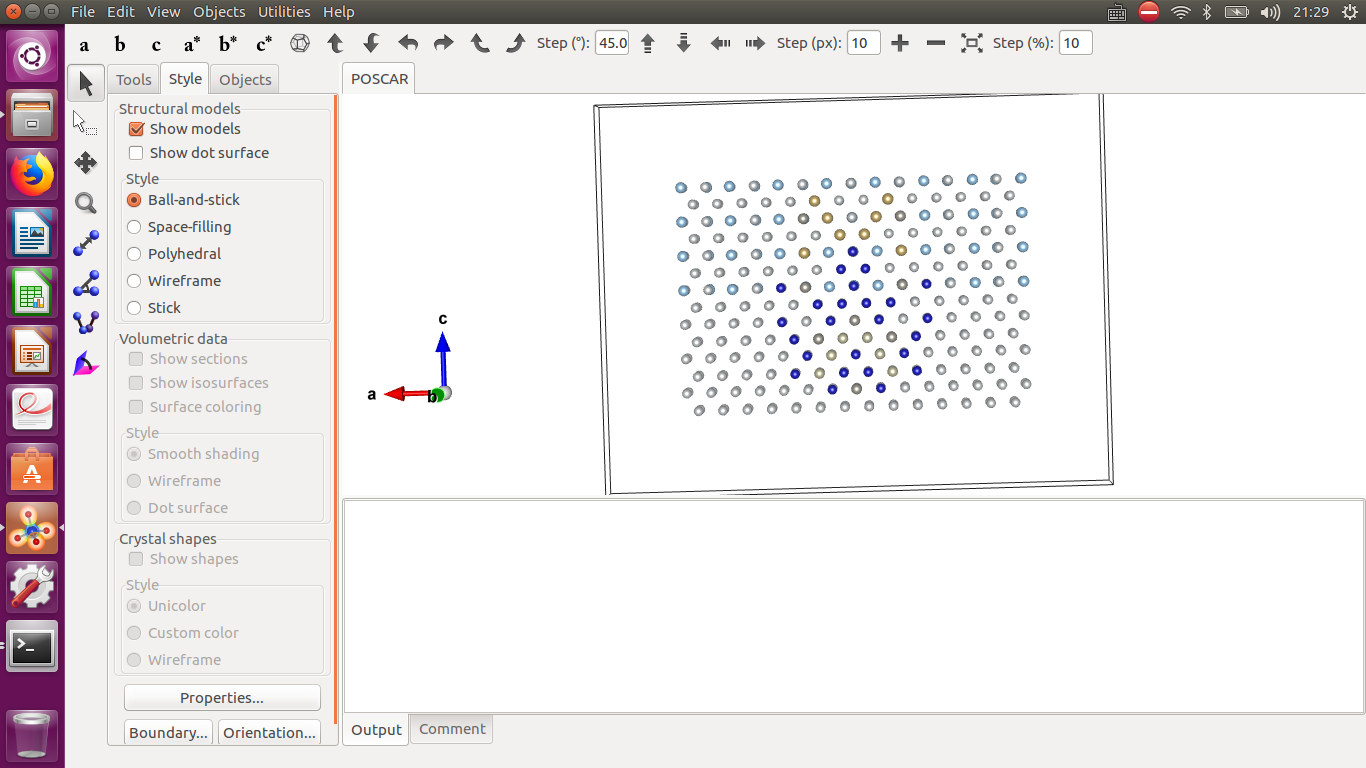
\includegraphics[height=3.45in,width=3.85in,viewport=580 120 1130 690,clip]{Ni3Al_orig-1.png}
\hspace{0.1in}
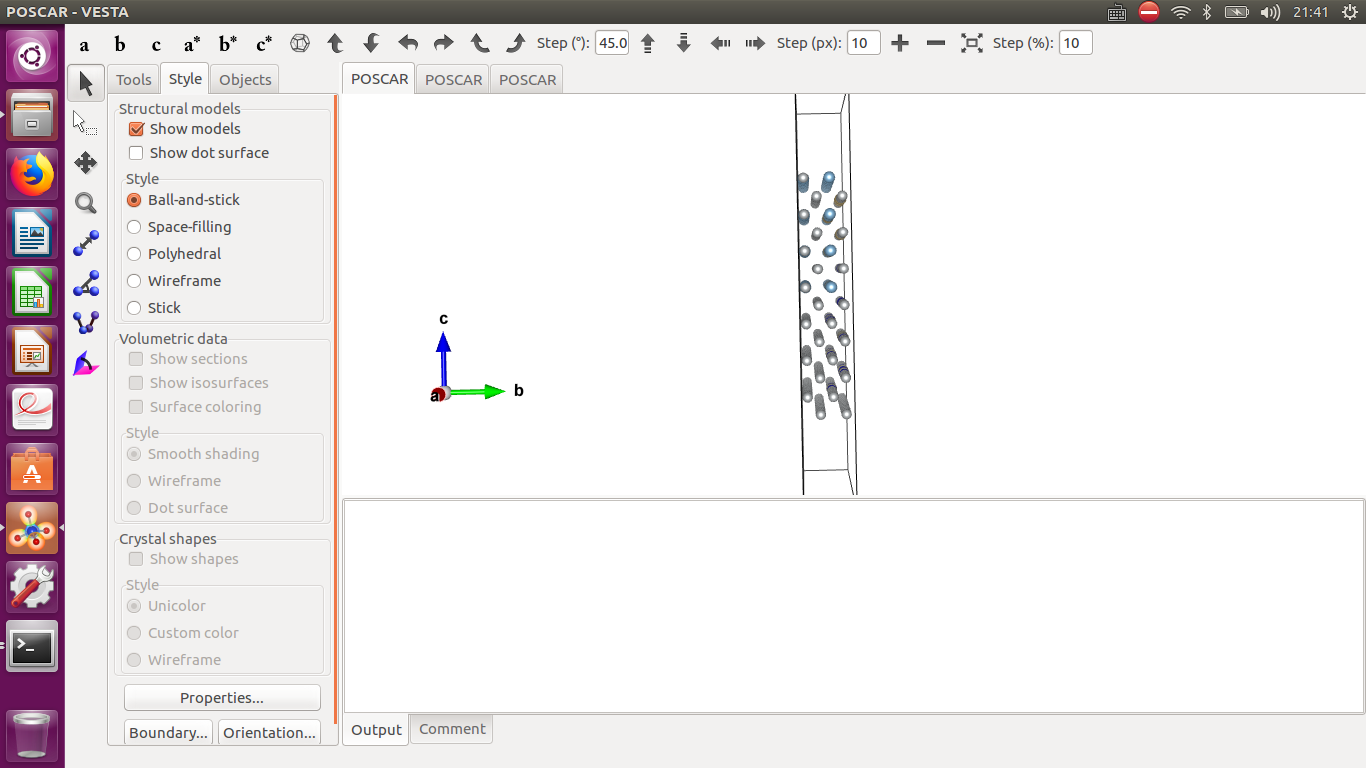
\includegraphics[height=3.45in,width=0.7in,viewport=770 120 880 690,clip]{Ni3Al_orig-2.png}
\caption{\small 初始六元系合金模型.}%(与文献\cite{EPJB33-47_2003}图1对比)
\label{Ni:Ni3Al_orig}
\end{figure}
\newpage
弛豫到133步后的晶格矢量变为
\begin{displaymath}
	\begin{pmatrix}
		55.4812057683920585   & 0.0000000000000000   & 0.0000000000000000 \\
     0.0000000000000000   & 3.8647052745834305  &  0.2335327946601230 \\
     0.0000000000000000   & 2.4658827600461595  & 43.6730869615263515
	\end{pmatrix}
\end{displaymath}
\begin{figure}[h!]
\centering
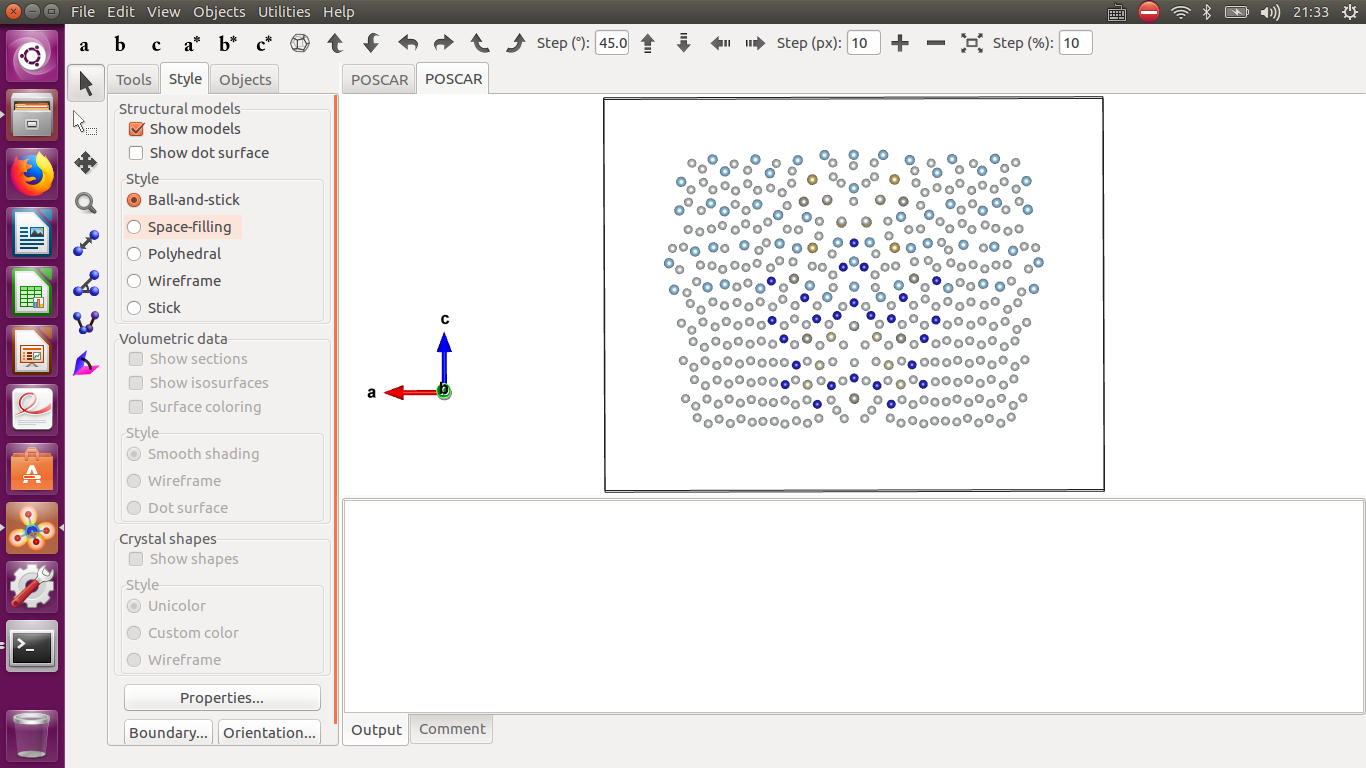
\includegraphics[height=3.55in,width=3.95in,viewport=580 120 1130 690,clip]{Ni3Al_mid-1.png}
\hspace{0.1in}
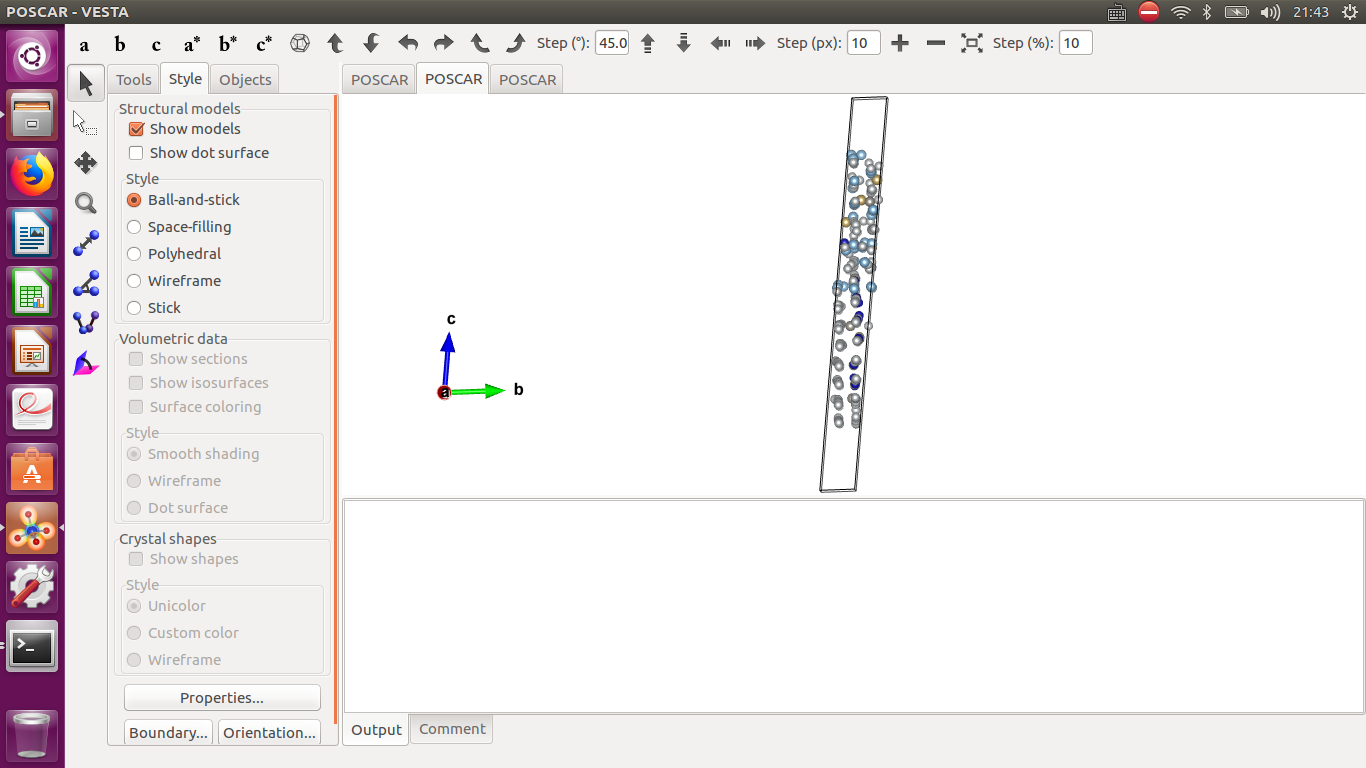
\includegraphics[height=3.55in,width=0.8in,viewport=800 120 920 690,clip]{Ni3Al_mid-2.png}
\caption{\small 六元系合金模型弛豫133步时的结构.}%(与文献\cite{EPJB33-47_2003}图1对比)
\label{Ni:Ni3Al_mid}
\end{figure}

\newpage
弛豫到第254步后的晶格矢量变为
\begin{displaymath}
	\begin{pmatrix}
		60.4691231290405256  & 0.0000000000000000   & 0.0000000000000000 \\
     0.0000000000000000   & 2.1267718192428737  &  0.1279079859326223 \\
     0.0000000000000000   & 0.0088038344936765  & 45.0815152841217781
	\end{pmatrix}
\end{displaymath}
\begin{figure}[h!]
\centering
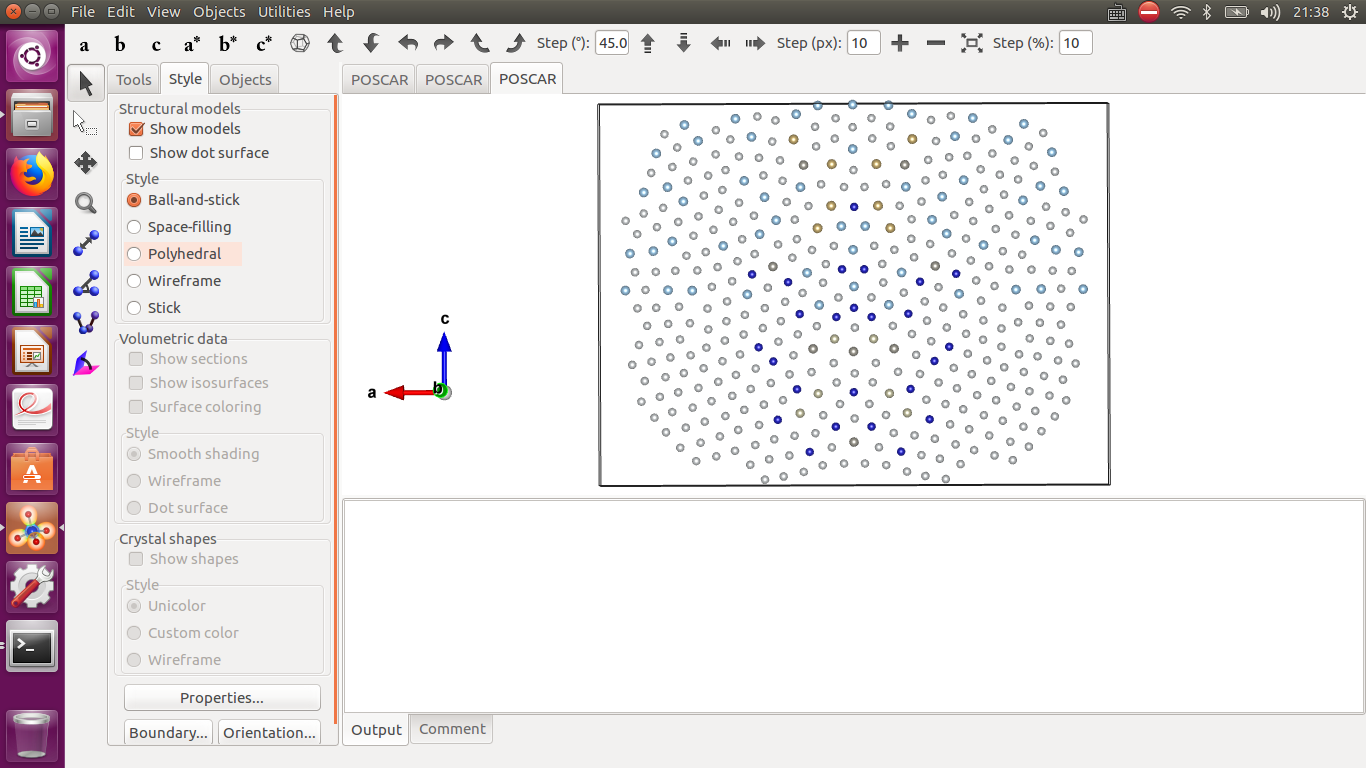
\includegraphics[height=3.55in,width=3.95in,viewport=580 120 1130 690,clip]{Ni3Al_fin-1.png}
\hspace{0.1in}
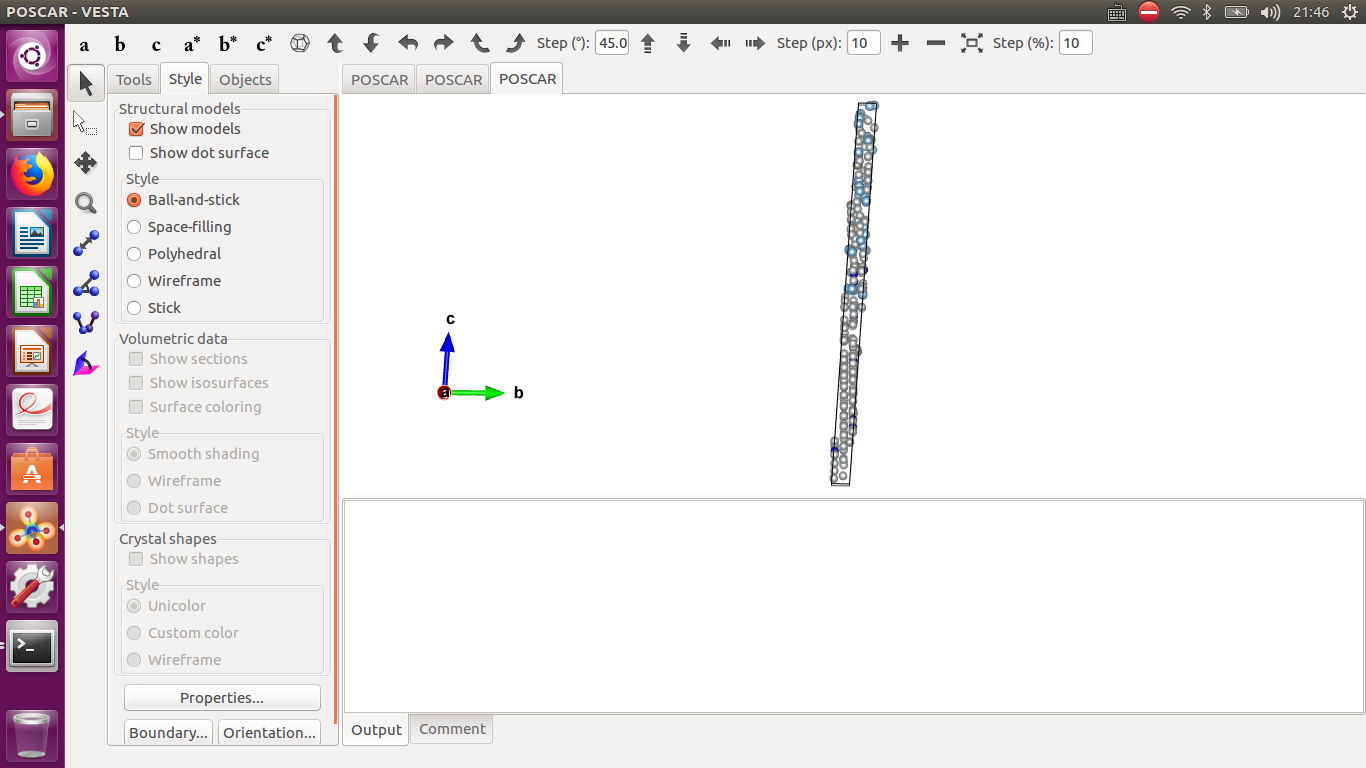
\includegraphics[height=3.55in,width=0.8in,viewport=800 120 920 690,clip]{Ni3Al_fin-2.png}
\caption{\small 六元系合金模型原子弛豫至254步后的结构.}%(与文献\cite{EPJB33-47_2003}图1对比)
\label{Ni:Ni3Al_fin}
\end{figure}
\newpage
计算过程中的参数设置:
\begin{itemize}
	\item \textrm{INCAR~}的参数设置
\begin{displaymath}
\boxed{
	\begin{aligned} 
		&\mathrm{STEM:~Ni\_Al\_Ta\_W\_Co\_Re~} \\
		&\mathrm{NWRITE=0} \\
		&\mathrm{ISTART=1} \\
		&\mathrm{SIGMA=0.2} \\
	&\mathrm{ISMEAR=1} \\
&\mathrm{ICHARG=2} \\
&\mathrm{\#ISPIN=2} \\
&\mathrm{ISIF=3} \\
&\mathrm{GGA=PE} \\
&\mathrm{ENCUT=300~eV} \\
&\mathrm{ALGO= F} \\
&\mathrm{\# LORBIT=11} \\
&\mathrm{LREAL=Auto} \\
&\mathrm{NELM=500} \\
&\mathrm{NELMIN=5} \\
&\mathrm{LWAVE = .FALSE.} \\
&\mathrm{LCHARG = .FALSE.} \\
&\mathrm{LVTOT = .FALSE.} \\
&\mathrm{NSW=300} \\
&\mathrm{\#VOSKOWN=1} \\
&\mathrm{EDIFF=1.0E-05} \\
&\mathrm{EDIFFG=-0.2} \\
&\mathrm{IBRION=2} \\
&\mathrm{LMAXMIX=4} \\
&\mathrm{AMIX=0.2} \\
&\mathrm{AMIN=0.01} \\
&\mathrm{NSIM=4} \\
&\mathrm{POTIM=0.2} \\
&\mathrm{\#ADDGRID= .True.} \\
&\mathrm{NPAR = 6} \\
&\mathrm{PREC=Accurate}
	\end{aligned}}
\end{displaymath}
	\item \textrm{KPOINTS~}的参数设置
\begin{displaymath}
\boxed{
	\begin{aligned}
		&\mathrm{Gamma-point~only}\\
		&\mathrm{0}\\
		&\mathrm{Monkhorst~Pack}\\
		&\mathrm{ 1~~1~~1}\\
		&\mathrm{ 0~~0~~0}
	\end{aligned}
}
\end{displaymath}
	\item \textrm{POTCAR}的参数版本
		\begin{displaymath}
\boxed{
	\begin{aligned}
		&\mathrm{POTCAR:~~~~PAW\_PBE~Ni~02Aug2007} \\                 
	&\mathrm{POTCAR:~~~~PAW\_PBE~Al~04Jan2001} \\               
	&\mathrm{POTCAR:~~~~PAW\_PBE~Ta~17Jan2003} \\                
	&\mathrm{POTCAR:~~~~PAW\_PBE~W~08Apr2002}  \\                 
	 &\mathrm{POTCAR:~~~~PAW\_PBE~Co~02Aug2007} \\                 
	 &\mathrm{POTCAR:~~~~PAW\_PBE~Re~17Jan2003}                  
 \end{aligned}}
		\end{displaymath}
	\item \textrm{POSCAR}的初始结构
		\begin{displaymath}
			\boxed{
				\begin{aligned}
					&\mathrm{Ni~Al~Ta~W~Co~Re} \\
&1.0 \\
& 52.1071 ~ ~    0 ~ ~       0 \\
&  0 ~ ~     5.0134 ~ ~    0 \\
&  0 ~ ~        0   ~ ~   40.3600 \\ 
&\mathrm{Ni~Al~Ta~W~Co~Re} \\
&303~56~8~8~25~6 \\
&\mathrm{Cartesian} \\
& 9.755479798 ~~   4.358769981 ~~   8.661500178  ~~\mathrm{F  ~~ F  ~~  F} \\ 
& 9.755479798 ~~   1.852069981 ~~   8.661500178  ~~\mathrm{F  ~~ F  ~~  F} \\ 
&43.595839788 ~~   0.598730008 ~~  31.704000083  ~~\mathrm{F  ~~ F  ~~  F} \\ 
&41.089150103 ~~   3.105419981 ~~  31.704000083  ~~\mathrm{F  ~~ F  ~~  F} \\ 
&12.262170005 ~~   4.358769981 ~~   8.661500178  ~~\mathrm{F  ~~ F  ~~  F} \\ 
&14.768860211 ~~   1.852069981 ~~   8.661500178  ~~\mathrm{F  ~~ F  ~~  F} \\ 
&38.582449997 ~~   0.598730008 ~~  31.704000083  ~~\mathrm{F  ~~ F  ~~  F} \\ 
&36.075759790 ~~   3.105419981 ~~  31.704000083  ~~\mathrm{F  ~~ F  ~~  F} \\ 
&17.275559796 ~~   4.358769981 ~~   8.661500178  ~~\mathrm{F  ~~ F  ~~  F} \\ 
&19.782250002 ~~   1.852069981 ~~   8.661500178  ~~\mathrm{F  ~~ F  ~~  F} \\ 
&33.569070105 ~~   0.598730008 ~~  31.704000083  ~~\mathrm{F  ~~ F  ~~  F} \\ 
&31.062369999 ~~   3.105419981 ~~  31.704000083  ~~\mathrm{F  ~~ F  ~~  F} \\ 
&22.288950109 ~~   4.358769981 ~~   8.661500178  ~~\mathrm{F  ~~ F  ~~  F} \\ 
&24.795639794 ~~   1.852069981 ~~   8.661500178  ~~\mathrm{F  ~~ F  ~~  F} \\ 
&28.555679793 ~~   0.598730008 ~~  31.704000083  ~~\mathrm{F  ~~ F  ~~  F} \\ 
&26.048990108 ~~   3.105419981 ~~  31.704000083  ~~\mathrm{F  ~~ F  ~~  F} \\ 
&27.302330000 ~~   4.358769981 ~~   8.661500178  ~~\mathrm{F  ~~ F  ~~  F} \\ 
&29.809030107 ~~   1.852069981 ~~   8.661500178  ~~\mathrm{F  ~~ F  ~~  F} \\ 
&23.542290001 ~~   0.598730008 ~~  31.704000083  ~~\mathrm{F  ~~ F  ~~  F} \\ 
&21.035599795 ~~   3.105419981 ~~  31.704000083  ~~\mathrm{F  ~~ F  ~~  F} \\ 
&32.315719792 ~~   4.358769981 ~~   8.661500178  ~~\mathrm{F  ~~ F  ~~  F} \\ 
&34.822409998 ~~   1.852069981 ~~   8.661500178  ~~\mathrm{F  ~~ F  ~~  F} \\ 
&18.528900210 ~~   0.598730008 ~~  31.704000083  ~~\mathrm{F  ~~ F  ~~  F} \\ 
&16.022210003 ~~   3.105419981 ~~  31.704000083  ~~\mathrm{F  ~~ F  ~~  F} \\ 
&37.329110104 ~~   4.358769981 ~~   8.661500178  ~~\mathrm{F  ~~ F  ~~  F} \\ 
&39.835799789 ~~   1.852069981 ~~   8.661500178  ~~\mathrm{F  ~~ F  ~~  F} \\ 
&13.515519797 ~~   0.598730008 ~~  31.704000083  ~~\mathrm{F  ~~ F  ~~  F} \\ 
&11.008820212 ~~   3.105419981 ~~  31.704000083  ~~\mathrm{F  ~~ F  ~~  F} \\ 
& 8.502130006 ~~   0.598730008 ~~  10.433999984  ~~\mathrm{F  ~~ F  ~~  F} \\ 
& 8.502130006 ~~   0.598730008 ~~  31.704000083  ~~\mathrm{F  ~~ F  ~~  F} \\ 
& 9.755479798 ~~   1.852069981 ~~  12.206500194  ~~\mathrm{T  ~~ T  ~~ T } \\ 
				\end{aligned}
			}
		\end{displaymath}
		\begin{displaymath}
			\boxed{
				\begin{aligned}
& 8.502130006 ~~   3.105419981 ~~  10.433999984  ~~\mathrm{F  ~~ F  ~~  F} \\ 
&42.342489996 ~~   4.358769981 ~~  29.931499873  ~~\mathrm{F  ~~ F  ~~  F} \\ 
&42.342489996 ~~   1.852069981 ~~  29.931499873  ~~\mathrm{F  ~~ F  ~~  F} \\ 
&43.595839788 ~~   0.598730008 ~~  28.159000066  ~~\mathrm{T  ~~ T  ~~ T } \\ 
&41.089150103 ~~   3.105419981 ~~  28.159000066  ~~\mathrm{T  ~~ T  ~~ T } \\ 
&12.262170005 ~~   4.358769981 ~~  12.206500194  ~~\mathrm{T  ~~ T  ~~ T } \\ 
&14.768860211 ~~   1.852069981 ~~  12.206500194  ~~\mathrm{T  ~~ T  ~~ T } \\ 
&39.835799789 ~~   1.852069981 ~~  29.931499873  ~~\mathrm{F  ~~ F  ~~  F} \\ 
&37.329110104 ~~   4.358769981 ~~  29.931499873  ~~\mathrm{F  ~~ F  ~~  F} \\ 
&39.835799789 ~~   4.358769981 ~~  29.931499873  ~~\mathrm{F  ~~ F  ~~  F} \\ 
&37.329110104 ~~   1.852069981 ~~  29.931499873  ~~\mathrm{F  ~~ F  ~~  F} \\ 
&38.582449997 ~~   0.598730008 ~~  28.159000066  ~~\mathrm{T  ~~ T  ~~ T } \\ 
&36.075759790 ~~   3.105419981 ~~  28.159000066  ~~\mathrm{T  ~~ T  ~~ T } \\ 
&17.275559796 ~~   4.358769981 ~~  12.206500194  ~~\mathrm{T  ~~ T  ~~ T } \\ 
&19.782250002 ~~   1.852069981 ~~  12.206500194  ~~\mathrm{T  ~~ T  ~~ T } \\ 
&34.822409998 ~~   1.852069981 ~~  29.931499873  ~~\mathrm{F  ~~ F  ~~  F} \\ 
&32.315719792 ~~   4.358769981 ~~  29.931499873  ~~\mathrm{F  ~~ F  ~~  F} \\ 
&34.822409998 ~~   4.358769981 ~~  29.931499873  ~~\mathrm{F  ~~ F  ~~  F} \\ 
&32.315719792 ~~   1.852069981 ~~  29.931499873  ~~\mathrm{F  ~~ F  ~~  F} \\ 
&33.569070105 ~~   0.598730008 ~~  28.159000066  ~~\mathrm{T  ~~ T  ~~ T } \\ 
&24.795639794 ~~   1.852069981 ~~  12.206500194  ~~\mathrm{T  ~~ T  ~~ T } \\ 
&29.809030107 ~~   1.852069981 ~~  29.931499873  ~~\mathrm{F  ~~ F  ~~  F} \\ 
&27.302330000 ~~   4.358769981 ~~  29.931499873  ~~\mathrm{F  ~~ F  ~~  F} \\ 
&27.302330000 ~~   1.852069981 ~~  29.931499873  ~~\mathrm{F  ~~ F  ~~  F} \\ 
&28.555679793 ~~   0.598730008 ~~  28.159000066  ~~\mathrm{T  ~~ T  ~~ T } \\ 
&26.048990108 ~~   3.105419981 ~~  28.159000066  ~~\mathrm{T  ~~ T  ~~ T } \\ 
&27.302330000 ~~   1.852069981 ~~  12.206500194  ~~\mathrm{T  ~~ T  ~~ T } \\ 
&18.528900210 ~~   3.105419981 ~~  10.433999984  ~~\mathrm{F  ~~ F  ~~  F} \\ 
&17.275559796 ~~   1.852069981 ~~  12.206500194  ~~\mathrm{T  ~~ T  ~~ T } \\ 
&31.062369999 ~~   3.105419981 ~~  10.433999984  ~~\mathrm{F  ~~ F  ~~  F} \\ 
&42.342489996 ~~   1.852069981 ~~   8.661500178  ~~\mathrm{F  ~~ F  ~~  F} \\ 
&14.768860211 ~~   4.358769981 ~~  12.206500194  ~~\mathrm{T  ~~ T  ~~ T } \\ 
&34.822409998 ~~   4.358769981 ~~  12.206500194  ~~\mathrm{T  ~~ T  ~~ T } \\ 
&39.835799789 ~~   4.358769981 ~~   8.661500178  ~~\mathrm{F  ~~ F  ~~  F} \\ 
&31.062369999 ~~   0.598730008 ~~  10.433999984  ~~\mathrm{F  ~~ F  ~~  F} \\ 
&33.569070105 ~~   3.105419981 ~~  10.433999984  ~~\mathrm{F  ~~ F  ~~  F} \\ 
&42.342489996 ~~   4.358769981 ~~   8.661500178  ~~\mathrm{F  ~~ F  ~~  F} \\ 
&38.582449997 ~~   0.598730008 ~~  10.433999984  ~~\mathrm{F  ~~ F  ~~  F} \\ 
&37.329110104 ~~   1.852069981 ~~  12.206500194  ~~\mathrm{T  ~~ T  ~~ T } \\ 
&28.555679793 ~~   0.598730008 ~~  10.433999984  ~~\mathrm{F  ~~ F  ~~  F} \\ 
				\end{aligned}
			}
		\end{displaymath}
		\begin{displaymath}
			\boxed{
				\begin{aligned}
& 9.755479798 ~~   4.358769981 ~~  12.206500194  ~~\mathrm{T  ~~ T  ~~ T } \\ 
&21.035599795 ~~   0.598730008 ~~  10.433999984  ~~\mathrm{F  ~~ F  ~~  F} \\ 
&11.008820212 ~~   3.105419981 ~~  10.433999984  ~~\mathrm{F  ~~ F  ~~  F} \\ 
&38.582449997 ~~   3.105419981 ~~  10.433999984  ~~\mathrm{F  ~~ F  ~~  F} \\ 
&41.089150103 ~~   3.105419981 ~~  10.433999984  ~~\mathrm{F  ~~ F  ~~  F} \\ 
&43.595839788 ~~   0.598730008 ~~  10.433999984  ~~\mathrm{F  ~~ F  ~~  F} \\ 
&42.342489996 ~~   1.852069981 ~~  12.206500194  ~~\mathrm{T  ~~ T  ~~ T } \\ 
&18.528900210 ~~   0.598730008 ~~  10.433999984  ~~\mathrm{F  ~~ F  ~~  F} \\ 
&16.022210003 ~~   3.105419981 ~~  10.433999984  ~~\mathrm{F  ~~ F  ~~  F} \\ 
&11.008820212 ~~   0.598730008 ~~  10.433999984  ~~\mathrm{F  ~~ F  ~~  F} \\ 
& 8.502130006 ~~   0.598730008 ~~  13.979000001  ~~\mathrm{T  ~~ T  ~~ T } \\ 
& 9.755479798 ~~   4.358769981 ~~  15.751499807  ~~\mathrm{T  ~~ T  ~~ T } \\ 
&29.809030107 ~~   4.358769981 ~~   8.661500178  ~~\mathrm{F  ~~ F  ~~  F} \\ 
&27.302330000 ~~   1.852069981 ~~   8.661500178  ~~\mathrm{F  ~~ F  ~~  F} \\ 
&11.008820212 ~~   3.105419981 ~~  13.979000001  ~~\mathrm{T  ~~ T  ~~ T } \\ 
&37.329110104 ~~   1.852069981 ~~   8.661500178  ~~\mathrm{F  ~~ F  ~~  F} \\ 
&12.262170005 ~~   1.852069981 ~~  15.751499807  ~~\mathrm{T  ~~ T  ~~ T } \\ 
&14.768860211 ~~   4.358769981 ~~  15.751499807  ~~\mathrm{T  ~~ T  ~~ T } \\ 
&36.075759790 ~~   3.105419981 ~~  10.433999984  ~~\mathrm{F  ~~ F  ~~  F} \\ 
&24.795639794 ~~   4.358769981 ~~   8.661500178  ~~\mathrm{F  ~~ F  ~~  F} \\ 
&11.008820212 ~~   0.598730008 ~~  13.979000001  ~~\mathrm{T  ~~ T  ~~ T } \\ 
&13.515519797 ~~   3.105419981 ~~  13.979000001  ~~\mathrm{T  ~~ T  ~~ T } \\ 
&16.022210003 ~~   3.105419981 ~~  13.979000001  ~~\mathrm{T  ~~ T  ~~ T } \\ 
&18.528900210 ~~   0.598730008 ~~  13.979000001  ~~\mathrm{T  ~~ T  ~~ T } \\ 
&22.288950109 ~~   1.852069981 ~~   8.661500178  ~~\mathrm{F  ~~ F  ~~  F} \\ 
&26.048990108 ~~   0.598730008 ~~  10.433999984  ~~\mathrm{F  ~~ F  ~~  F} \\ 
&19.782250002 ~~   4.358769981 ~~   8.661500178  ~~\mathrm{F  ~~ F  ~~  F} \\ 
&16.022210003 ~~   0.598730008 ~~  13.979000001  ~~\mathrm{T  ~~ T  ~~ T } \\ 
&18.528900210 ~~   3.105419981 ~~  13.979000001  ~~\mathrm{T  ~~ T  ~~ T } \\ 
&23.542290001 ~~   0.598730008 ~~  13.979000001  ~~\mathrm{T  ~~ T  ~~ T } \\ 
&22.288950109 ~~   1.852069981 ~~  15.751499807  ~~\mathrm{T  ~~ T  ~~ T } \\ 
&17.275559796 ~~   1.852069981 ~~   8.661500178  ~~\mathrm{F  ~~ F  ~~  F} \\ 
&22.288950109 ~~   1.852069981 ~~  12.206500194  ~~\mathrm{T  ~~ T  ~~ T } \\ 
&23.542290001 ~~   0.598730008 ~~  10.433999984  ~~\mathrm{F  ~~ F  ~~  F} \\ 
&21.035599795 ~~   3.105419981 ~~  10.433999984  ~~\mathrm{F  ~~ F  ~~  F} \\ 
&28.555679793 ~~   0.598730008 ~~  13.979000001  ~~\mathrm{T  ~~ T  ~~ T } \\ 
&27.302330000 ~~   1.852069981 ~~  15.751499807  ~~\mathrm{T  ~~ T  ~~ T } \\ 
&12.262170005 ~~   1.852069981 ~~   8.661500178  ~~\mathrm{F  ~~ F  ~~  F} \\ 
&13.515519797 ~~   3.105419981 ~~  10.433999984  ~~\mathrm{F  ~~ F  ~~  F} \\ 
&26.048990108 ~~   0.598730008 ~~  13.979000001  ~~\mathrm{T  ~~ T  ~~ T } \\ 
				\end{aligned}
			}
		\end{displaymath}
		\begin{displaymath}
			\boxed{
				\begin{aligned}
&33.569070105 ~~   0.598730008 ~~  13.979000001  ~~\mathrm{T  ~~ T  ~~ T } \\ 
&32.315719792 ~~   1.852069981 ~~  15.751499807  ~~\mathrm{T  ~~ T  ~~ T } \\ 
&34.822409998 ~~   4.358769981 ~~  15.751499807  ~~\mathrm{T  ~~ T  ~~ T } \\ 
&21.035599795 ~~   0.598730008 ~~  13.979000001  ~~\mathrm{T  ~~ T  ~~ T } \\ 
&31.062369999 ~~   0.598730008 ~~  13.979000001  ~~\mathrm{T  ~~ T  ~~ T } \\ 
&33.569070105 ~~   3.105419981 ~~  13.979000001  ~~\mathrm{T  ~~ T  ~~ T } \\ 
&36.075759790 ~~   3.105419981 ~~  13.979000001  ~~\mathrm{T  ~~ T  ~~ T } \\ 
&38.582449997 ~~   0.598730008 ~~  13.979000001  ~~\mathrm{T  ~~ T  ~~ T } \\ 
&37.329110104 ~~   1.852069981 ~~  15.751499807  ~~\mathrm{T  ~~ T  ~~ T } \\ 
&39.835799789 ~~   4.358769981 ~~  15.751499807  ~~\mathrm{T  ~~ T  ~~ T } \\ 
&17.275559796 ~~   1.852069981 ~~  15.751499807  ~~\mathrm{T  ~~ T  ~~ T } \\ 
&36.075759790 ~~   0.598730008 ~~  13.979000001  ~~\mathrm{T  ~~ T  ~~ T } \\ 
&38.582449997 ~~   3.105419981 ~~  13.979000001  ~~\mathrm{T  ~~ T  ~~ T } \\ 
&41.089150103 ~~   3.105419981 ~~  13.979000001  ~~\mathrm{T  ~~ T  ~~ T } \\ 
&43.595839788 ~~   0.598730008 ~~  13.979000001  ~~\mathrm{T  ~~ T  ~~ T } \\ 
&42.342489996 ~~   1.852069981 ~~  15.751499807  ~~\mathrm{T  ~~ T  ~~ T } \\ 
&42.342489996 ~~   4.358769981 ~~  15.751499807  ~~\mathrm{T  ~~ T  ~~ T } \\ 
&13.515519797 ~~   0.598730008 ~~  13.979000001  ~~\mathrm{T  ~~ T  ~~ T } \\ 
&43.595839788 ~~   3.105419981 ~~  13.979000001  ~~\mathrm{T  ~~ T  ~~ T } \\ 
& 8.502130006 ~~   0.598730008 ~~  17.524000017  ~~\mathrm{T  ~~ T  ~~ T } \\ 
& 9.755479798 ~~   4.358769981 ~~  19.296499824  ~~\mathrm{T  ~~ T  ~~ T } \\ 
&43.595839788 ~~   3.105419981 ~~  10.433999984  ~~\mathrm{F  ~~ F  ~~  F} \\ 
&42.342489996 ~~   4.358769981 ~~  12.206500194  ~~\mathrm{T  ~~ T  ~~ T } \\ 
&11.008820212 ~~   3.105419981 ~~  17.524000017  ~~\mathrm{T  ~~ T  ~~ T } \\ 
&13.515519797 ~~   0.598730008 ~~  17.524000017  ~~\mathrm{T  ~~ T  ~~ T } \\ 
&12.262170005 ~~   1.852069981 ~~  19.296499824  ~~\mathrm{T  ~~ T  ~~ T } \\ 
&14.768860211 ~~   4.358769981 ~~  19.296499824  ~~\mathrm{T  ~~ T  ~~ T } \\ 
&36.075759790 ~~   0.598730008 ~~  10.433999984  ~~\mathrm{F  ~~ F  ~~  F} \\ 
&39.835799789 ~~   4.358769981 ~~  12.206500194  ~~\mathrm{T  ~~ T  ~~ T } \\ 
&11.008820212 ~~   0.598730008 ~~  17.524000017  ~~\mathrm{T  ~~ T  ~~ T } \\ 
&13.515519797 ~~   3.105419981 ~~  17.524000017  ~~\mathrm{T  ~~ T  ~~ T } \\ 
&16.022210003 ~~   3.105419981 ~~  17.524000017  ~~\mathrm{T  ~~ T  ~~ T } \\ 
&18.528900210 ~~   0.598730008 ~~  17.524000017  ~~\mathrm{T  ~~ T  ~~ T } \\ 
&17.275559796 ~~   1.852069981 ~~  19.296499824  ~~\mathrm{T  ~~ T  ~~ T } \\ 
&19.782250002 ~~   4.358769981 ~~  19.296499824  ~~\mathrm{T  ~~ T  ~~ T } \\ 
&32.315719792 ~~   1.852069981 ~~  12.206500194  ~~\mathrm{T  ~~ T  ~~ T } \\ 
&33.569070105 ~~   0.598730008 ~~  10.433999984  ~~\mathrm{F  ~~ F  ~~  F} \\ 
&16.022210003 ~~   0.598730008 ~~  17.524000017  ~~\mathrm{T  ~~ T  ~~ T } \\ 
&21.035599795 ~~   3.105419981 ~~  17.524000017  ~~\mathrm{T  ~~ T  ~~ T } \\ 
				\end{aligned}
			}
		\end{displaymath}
		\begin{displaymath}
			\boxed{
				\begin{aligned}
&23.542290001 ~~   0.598730008 ~~  17.524000017  ~~\mathrm{T  ~~ T  ~~ T } \\ 
&22.288950109 ~~   1.852069981 ~~  19.296499824  ~~\mathrm{T  ~~ T  ~~ T } \\ 
&21.035599795 ~~   0.598730008 ~~  17.524000017  ~~\mathrm{T  ~~ T  ~~ T } \\ 
&28.555679793 ~~   0.598730008 ~~  17.524000017  ~~\mathrm{T  ~~ T  ~~ T } \\ 
&27.302330000 ~~   1.852069981 ~~  19.296499824  ~~\mathrm{T  ~~ T  ~~ T } \\ 
&16.022210003 ~~   0.598730008 ~~  10.433999984  ~~\mathrm{F  ~~ F  ~~  F} \\ 
&26.048990108 ~~   0.598730008 ~~  17.524000017  ~~\mathrm{T  ~~ T  ~~ T } \\ 
&31.062369999 ~~   3.105419981 ~~  17.524000017  ~~\mathrm{T  ~~ T  ~~ T } \\ 
&33.569070105 ~~   0.598730008 ~~  17.524000017  ~~\mathrm{T  ~~ T  ~~ T } \\ 
&32.315719792 ~~   1.852069981 ~~  19.296499824  ~~\mathrm{T  ~~ T  ~~ T } \\ 
&34.822409998 ~~   4.358769981 ~~  19.296499824  ~~\mathrm{T  ~~ T  ~~ T } \\ 
&12.262170005 ~~   1.852069981 ~~  12.206500194  ~~\mathrm{T  ~~ T  ~~ T } \\ 
&13.515519797 ~~   0.598730008 ~~  10.433999984  ~~\mathrm{F  ~~ F  ~~  F} \\ 
&31.062369999 ~~   0.598730008 ~~  17.524000017  ~~\mathrm{T  ~~ T  ~~ T } \\ 
&36.075759790 ~~   3.105419981 ~~  17.524000017  ~~\mathrm{T  ~~ T  ~~ T } \\ 
&38.582449997 ~~   0.598730008 ~~  17.524000017  ~~\mathrm{T  ~~ T  ~~ T } \\ 
&37.329110104 ~~   1.852069981 ~~  19.296499824  ~~\mathrm{T  ~~ T  ~~ T } \\ 
&39.835799789 ~~   4.358769981 ~~  19.296499824  ~~\mathrm{T  ~~ T  ~~ T } \\ 
&34.822409998 ~~   4.358769981 ~~   8.661500178  ~~\mathrm{F  ~~ F  ~~  F} \\ 
&32.315719792 ~~   1.852069981 ~~   8.661500178  ~~\mathrm{F  ~~ F  ~~  F} \\ 
&36.075759790 ~~   0.598730008 ~~  17.524000017  ~~\mathrm{T  ~~ T  ~~ T } \\ 
&38.582449997 ~~   3.105419981 ~~  17.524000017  ~~\mathrm{T  ~~ T  ~~ T } \\ 
&41.089150103 ~~   3.105419981 ~~  17.524000017  ~~\mathrm{T  ~~ T  ~~ T } \\ 
&43.595839788 ~~   0.598730008 ~~  17.524000017  ~~\mathrm{T  ~~ T  ~~ T } \\ 
&42.342489996 ~~   1.852069981 ~~  19.296499824  ~~\mathrm{T  ~~ T  ~~ T } \\ 
&42.342489996 ~~   4.358769981 ~~  19.296499824  ~~\mathrm{T  ~~ T  ~~ T } \\ 
&14.768860211 ~~   4.358769981 ~~   8.661500178  ~~\mathrm{F  ~~ F  ~~  F} \\ 
&43.595839788 ~~   3.105419981 ~~  17.524000017  ~~\mathrm{T  ~~ T  ~~ T } \\ 
& 8.502130006 ~~   0.598730008 ~~  21.069000034  ~~\mathrm{T  ~~ T  ~~ T } \\ 
& 9.755479798 ~~   4.358769981 ~~  22.841499840  ~~\mathrm{T  ~~ T  ~~ T } \\ 
& 9.755479798 ~~   1.852069981 ~~  22.841499840  ~~\mathrm{T  ~~ T  ~~ T } \\ 
&41.089150103 ~~   0.598730008 ~~  17.524000017  ~~\mathrm{T  ~~ T  ~~ T } \\ 
&11.008820212 ~~   3.105419981 ~~  21.069000034  ~~\mathrm{T  ~~ T  ~~ T } \\ 
&13.515519797 ~~   0.598730008 ~~  21.069000034  ~~\mathrm{T  ~~ T  ~~ T } \\ 
&12.262170005 ~~   1.852069981 ~~  22.841499840  ~~\mathrm{T  ~~ T  ~~ T } \\ 
&14.768860211 ~~   4.358769981 ~~  22.841499840  ~~\mathrm{T  ~~ T  ~~ T } \\ 
&12.262170005 ~~   4.358769981 ~~  22.841499840  ~~\mathrm{T  ~~ T  ~~ T } \\ 
&14.768860211 ~~   1.852069981 ~~  22.841499840  ~~\mathrm{T  ~~ T  ~~ T } \\ 
&39.835799789 ~~   1.852069981 ~~  19.296499824  ~~\mathrm{T  ~~ T  ~~ T } \\ 
				\end{aligned}
			}
		\end{displaymath}
		\begin{displaymath}
			\boxed{
				\begin{aligned}
&37.329110104 ~~   4.358769981 ~~  19.296499824  ~~\mathrm{T  ~~ T  ~~ T } \\ 
&16.022210003 ~~   3.105419981 ~~  21.069000034  ~~\mathrm{T  ~~ T  ~~ T } \\ 
&18.528900210 ~~   0.598730008 ~~  21.069000034  ~~\mathrm{T  ~~ T  ~~ T } \\ 
&17.275559796 ~~   1.852069981 ~~  22.841499840  ~~\mathrm{T  ~~ T  ~~ T } \\ 
&19.782250002 ~~   4.358769981 ~~  22.841499840  ~~\mathrm{T  ~~ T  ~~ T } \\ 
&17.275559796 ~~   4.358769981 ~~  22.841499840  ~~\mathrm{T  ~~ T  ~~ T } \\ 
&19.782250002 ~~   1.852069981 ~~  22.841499840  ~~\mathrm{T  ~~ T  ~~ T } \\ 
&34.822409998 ~~   1.852069981 ~~  19.296499824  ~~\mathrm{T  ~~ T  ~~ T } \\ 
&32.315719792 ~~   4.358769981 ~~  19.296499824  ~~\mathrm{T  ~~ T  ~~ T } \\ 
&23.542290001 ~~   0.598730008 ~~  21.069000034  ~~\mathrm{T  ~~ T  ~~ T } \\ 
&22.288950109 ~~   1.852069981 ~~  22.841499840  ~~\mathrm{T  ~~ T  ~~ T } \\ 
&22.288950109 ~~   4.358769981 ~~  22.841499840  ~~\mathrm{T  ~~ T  ~~ T } \\ 
&24.795639794 ~~   1.852069981 ~~  22.841499840  ~~\mathrm{T  ~~ T  ~~ T } \\ 
&29.809030107 ~~   1.852069981 ~~  19.296499824  ~~\mathrm{T  ~~ T  ~~ T } \\ 
&28.555679793 ~~   0.598730008 ~~  21.069000034  ~~\mathrm{T  ~~ T  ~~ T } \\ 
&27.302330000 ~~   1.852069981 ~~  22.841499840  ~~\mathrm{T  ~~ T  ~~ T } \\ 
&29.809030107 ~~   4.358769981 ~~  22.841499840  ~~\mathrm{T  ~~ T  ~~ T } \\ 
&29.809030107 ~~   1.852069981 ~~  22.841499840  ~~\mathrm{T  ~~ T  ~~ T } \\ 
&24.795639794 ~~   1.852069981 ~~  19.296499824  ~~\mathrm{T  ~~ T  ~~ T } \\ 
&33.569070105 ~~   0.598730008 ~~  21.069000034  ~~\mathrm{T  ~~ T  ~~ T } \\ 
&32.315719792 ~~   1.852069981 ~~  22.841499840  ~~\mathrm{T  ~~ T  ~~ T } \\ 
&34.822409998 ~~   4.358769981 ~~  22.841499840  ~~\mathrm{T  ~~ T  ~~ T } \\ 
&32.315719792 ~~   4.358769981 ~~  22.841499840  ~~\mathrm{T  ~~ T  ~~ T } \\ 
&34.822409998 ~~   1.852069981 ~~  22.841499840  ~~\mathrm{T  ~~ T  ~~ T } \\ 
&19.782250002 ~~   1.852069981 ~~  19.296499824  ~~\mathrm{T  ~~ T  ~~ T } \\ 
&17.275559796 ~~   4.358769981 ~~  19.296499824  ~~\mathrm{T  ~~ T  ~~ T } \\ 
&36.075759790 ~~   3.105419981 ~~  21.069000034  ~~\mathrm{T  ~~ T  ~~ T } \\ 
&38.582449997 ~~   0.598730008 ~~  21.069000034  ~~\mathrm{T  ~~ T  ~~ T } \\ 
&37.329110104 ~~   1.852069981 ~~  22.841499840  ~~\mathrm{T  ~~ T  ~~ T } \\ 
&39.835799789 ~~   4.358769981 ~~  22.841499840  ~~\mathrm{T  ~~ T  ~~ T } \\ 
&37.329110104 ~~   4.358769981 ~~  22.841499840  ~~\mathrm{T  ~~ T  ~~ T } \\ 
&39.835799789 ~~   1.852069981 ~~  22.841499840  ~~\mathrm{T  ~~ T  ~~ T } \\ 
&14.768860211 ~~   1.852069981 ~~  19.296499824  ~~\mathrm{T  ~~ T  ~~ T } \\
&12.262170005 ~~   4.358769981 ~~  19.296499824  ~~\mathrm{T  ~~ T  ~~ T } \\ 
&41.089150103 ~~   3.105419981 ~~  21.069000034  ~~\mathrm{T  ~~ T  ~~ T } \\ 
&43.595839788 ~~   0.598730008 ~~  21.069000034  ~~\mathrm{T  ~~ T  ~~ T } \\ 
&42.342489996 ~~   1.852069981 ~~  22.841499840  ~~\mathrm{T  ~~ T  ~~ T } \\ 
&42.342489996 ~~   4.358769981 ~~  22.841499840  ~~\mathrm{T  ~~ T  ~~ T } \\ 
& 8.502130006 ~~   3.105419981 ~~  17.524000017  ~~\mathrm{T  ~~ T  ~~ T } \\ 
& 9.755479798 ~~   1.852069981 ~~  19.296499824  ~~\mathrm{T  ~~ T  ~~ T } \\ 
& 8.502130006 ~~   0.598730008 ~~  24.614000050  ~~\mathrm{T  ~~ T  ~~ T } \\ 
& 9.755479798 ~~   4.358769981 ~~  26.386499856  ~~\mathrm{T  ~~ T  ~~ T } \\ 
& 9.755479798 ~~   1.852069981 ~~  26.386499856  ~~\mathrm{T  ~~ T  ~~ T } \\ 
&41.089150103 ~~   0.598730008 ~~  13.979000001  ~~\mathrm{T  ~~ T  ~~ T } \\ 
&11.008820212 ~~   3.105419981 ~~  24.614000050  ~~\mathrm{T  ~~ T  ~~ T } \\ 
				\end{aligned}
			}
		\end{displaymath}
		\begin{displaymath}
			\boxed{
				\begin{aligned}
&13.515519797 ~~   0.598730008 ~~  24.614000050  ~~\mathrm{T  ~~ T  ~~ T } \\ 
&12.262170005 ~~   1.852069981 ~~  26.386499856  ~~\mathrm{T  ~~ T  ~~ T } \\ 
&14.768860211 ~~   4.358769981 ~~  26.386499856  ~~\mathrm{T  ~~ T  ~~ T } \\ 
&12.262170005 ~~   4.358769981 ~~  26.386499856  ~~\mathrm{T  ~~ T  ~~ T } \\ 
&14.768860211 ~~   1.852069981 ~~  26.386499856  ~~\mathrm{T  ~~ T  ~~ T } \\ 
&39.835799789 ~~   1.852069981 ~~  15.751499807  ~~\mathrm{T  ~~ T  ~~ T } \\ 
&37.329110104 ~~   4.358769981 ~~  15.751499807  ~~\mathrm{T  ~~ T  ~~ T } \\ 
&16.022210003 ~~   3.105419981 ~~  24.614000050  ~~\mathrm{T  ~~ T  ~~ T } \\ 
&18.528900210 ~~   0.598730008 ~~  24.614000050  ~~\mathrm{T  ~~ T  ~~ T } \\ 
&17.275559796 ~~   1.852069981 ~~  26.386499856  ~~\mathrm{T  ~~ T  ~~ T } \\ 
&19.782250002 ~~   4.358769981 ~~  26.386499856  ~~\mathrm{T  ~~ T  ~~ T } \\ 
&17.275559796 ~~   4.358769981 ~~  26.386499856  ~~\mathrm{T  ~~ T  ~~ T } \\ 
&19.782250002 ~~   1.852069981 ~~  26.386499856  ~~\mathrm{T  ~~ T  ~~ T } \\ 
&34.822409998 ~~   1.852069981 ~~  15.751499807  ~~\mathrm{T  ~~ T  ~~ T } \\ 
&23.542290001 ~~   0.598730008 ~~  24.614000050  ~~\mathrm{T  ~~ T  ~~ T } \\ 
&22.288950109 ~~   1.852069981 ~~  26.386499856  ~~\mathrm{T  ~~ T  ~~ T } \\ 
&22.288950109 ~~   4.358769981 ~~  26.386499856  ~~\mathrm{T  ~~ T  ~~ T } \\ 
&24.795639794 ~~   1.852069981 ~~  26.386499856  ~~\mathrm{T  ~~ T  ~~ T } \\ 
&29.809030107 ~~   1.852069981 ~~  15.751499807  ~~\mathrm{T  ~~ T  ~~ T } \\ 
&28.555679793 ~~   0.598730008 ~~  24.614000050  ~~\mathrm{T  ~~ T  ~~ T } \\ 
&27.302330000 ~~   1.852069981 ~~  26.386499856  ~~\mathrm{T  ~~ T  ~~ T } \\ 
&29.809030107 ~~   4.358769981 ~~  26.386499856  ~~\mathrm{T  ~~ T  ~~ T } \\ 
&29.809030107 ~~   1.852069981 ~~  26.386499856  ~~\mathrm{T  ~~ T  ~~ T } \\ 
&24.795639794 ~~   1.852069981 ~~  15.751499807  ~~\mathrm{T  ~~ T  ~~ T } \\ 
&33.569070105 ~~   0.598730008 ~~  24.614000050  ~~\mathrm{T  ~~ T  ~~ T } \\ 
&32.315719792 ~~   1.852069981 ~~  26.386499856  ~~\mathrm{T  ~~ T  ~~ T } \\ 
&34.822409998 ~~   4.358769981 ~~  26.386499856  ~~\mathrm{T  ~~ T  ~~ T } \\ 
&32.315719792 ~~   4.358769981 ~~  26.386499856  ~~\mathrm{T  ~~ T  ~~ T } \\ 
&34.822409998 ~~   1.852069981 ~~  26.386499856  ~~\mathrm{T  ~~ T  ~~ T } \\ 
&19.782250002 ~~   1.852069981 ~~  15.751499807  ~~\mathrm{T  ~~ T  ~~ T } \\ 
&17.275559796 ~~   4.358769981 ~~  15.751499807  ~~\mathrm{T  ~~ T  ~~ T } \\ 
&36.075759790 ~~   3.105419981 ~~  24.614000050  ~~\mathrm{T  ~~ T  ~~ T } \\ 
&38.582449997 ~~   0.598730008 ~~  24.614000050  ~~\mathrm{T  ~~ T  ~~ T } \\ 
&37.329110104 ~~   1.852069981 ~~  26.386499856  ~~\mathrm{T  ~~ T  ~~ T } \\ 
&39.835799789 ~~   4.358769981 ~~  26.386499856  ~~\mathrm{T  ~~ T  ~~ T } \\ 
				\end{aligned}
			}
		\end{displaymath}
		\begin{displaymath}
			\boxed{
				\begin{aligned}
&37.329110104 ~~   4.358769981 ~~  26.386499856  ~~\mathrm{T  ~~ T  ~~ T } \\ 
&39.835799789 ~~   1.852069981 ~~  26.386499856  ~~\mathrm{T  ~~ T  ~~ T } \\ 
&14.768860211 ~~   1.852069981 ~~  15.751499807  ~~\mathrm{T  ~~ T  ~~ T } \\ 
&12.262170005 ~~   4.358769981 ~~  15.751499807  ~~\mathrm{T  ~~ T  ~~ T } \\ 
&41.089150103 ~~   3.105419981 ~~  24.614000050  ~~\mathrm{T  ~~ T  ~~ T } \\ 
&43.595839788 ~~   0.598730008 ~~  24.614000050  ~~\mathrm{T  ~~ T  ~~ T } \\ 
&42.342489996 ~~   1.852069981 ~~  26.386499856  ~~\mathrm{T  ~~ T  ~~ T } \\ 
&42.342489996 ~~   4.358769981 ~~  26.386499856  ~~\mathrm{T  ~~ T  ~~ T } \\ 
& 8.502130006 ~~   3.105419981 ~~  13.979000001  ~~\mathrm{T  ~~ T  ~~ T } \\ 
& 9.755479798 ~~   1.852069981 ~~  15.751499807  ~~\mathrm{T  ~~ T  ~~ T } \\ 
& 8.502130006 ~~   0.598730008 ~~  28.159000066  ~~\mathrm{T  ~~ T  ~~ T } \\ 
& 9.755479798 ~~   4.358769981 ~~  29.931499873  ~~\mathrm{F  ~~ F  ~~  F} \\ 
& 9.755479798 ~~   1.852069981 ~~  29.931499873  ~~\mathrm{F  ~~ F  ~~  F} \\ 
&41.089150103 ~~   0.598730008 ~~  10.433999984  ~~\mathrm{F  ~~ F  ~~  F} \\ 
&11.008820212 ~~   3.105419981 ~~  28.159000066  ~~\mathrm{T  ~~ T  ~~ T } \\ 
&13.515519797 ~~   0.598730008 ~~  28.159000066  ~~\mathrm{T  ~~ T  ~~ T } \\ 
&12.262170005 ~~   1.852069981 ~~  29.931499873  ~~\mathrm{F  ~~ F  ~~  F} \\ 
&14.768860211 ~~   4.358769981 ~~  29.931499873  ~~\mathrm{F  ~~ F  ~~  F} \\ 
&12.262170005 ~~   4.358769981 ~~  29.931499873  ~~\mathrm{F  ~~ F  ~~  F} \\ 
&14.768860211 ~~   1.852069981 ~~  29.931499873  ~~\mathrm{F  ~~ F  ~~  F} \\ 
&39.835799789 ~~   1.852069981 ~~  12.206500194  ~~\mathrm{T  ~~ T  ~~ T } \\ 
&37.329110104 ~~   4.358769981 ~~  12.206500194  ~~\mathrm{T  ~~ T  ~~ T } \\ 
&16.022210003 ~~   3.105419981 ~~  28.159000066  ~~\mathrm{T  ~~ T  ~~ T } \\ 
&18.528900210 ~~   0.598730008 ~~  28.159000066  ~~\mathrm{T  ~~ T  ~~ T } \\ 
&17.275559796 ~~   1.852069981 ~~  29.931499873  ~~\mathrm{F  ~~ F  ~~  F} \\ 
&19.782250002 ~~   4.358769981 ~~  29.931499873  ~~\mathrm{F  ~~ F  ~~  F} \\ 
&17.275559796 ~~   4.358769981 ~~  29.931499873  ~~\mathrm{F  ~~ F  ~~  F} \\ 
&19.782250002 ~~   1.852069981 ~~  29.931499873  ~~\mathrm{F  ~~ F  ~~  F} \\ 
&34.822409998 ~~   1.852069981 ~~  12.206500194  ~~\mathrm{T  ~~ T  ~~ T } \\ 
				\end{aligned}
			}
		\end{displaymath}
		\begin{displaymath}
			\boxed{
				\begin{aligned}
&23.542290001 ~~   0.598730008 ~~  28.159000066  ~~\mathrm{T  ~~ T  ~~ T } \\ 
&22.288950109 ~~   1.852069981 ~~  29.931499873  ~~\mathrm{F  ~~ F  ~~  F} \\ 
&24.795639794 ~~   4.358769981 ~~  29.931499873  ~~\mathrm{F  ~~ F  ~~  F} \\ 
&24.795639794 ~~   1.852069981 ~~  29.931499873  ~~\mathrm{F  ~~ F  ~~  F} \\ 
&29.809030107 ~~   1.852069981 ~~  12.206500194  ~~\mathrm{T  ~~ T  ~~ T } \\ 
&33.569070105 ~~   3.105419981 ~~  24.614000050  ~~\mathrm{T  ~~ T  ~~ T } \\ 
&13.515519797 ~~   3.105419981 ~~  24.614000050  ~~\mathrm{T  ~~ T  ~~ T } \\ 
&13.515519797 ~~   3.105419981 ~~  28.159000066  ~~\mathrm{T  ~~ T  ~~ T } \\ 
&26.048990108 ~~   0.598730008 ~~  21.069000034  ~~\mathrm{T  ~~ T  ~~ T } \\ 
&26.048990108 ~~   0.598730008 ~~  28.159000066  ~~\mathrm{T  ~~ T  ~~ T } \\ 
&38.582449997 ~~   3.105419981 ~~  21.069000034  ~~\mathrm{T  ~~ T  ~~ T } \\ 
&18.528900210 ~~   3.105419981 ~~  28.159000066  ~~\mathrm{T  ~~ T  ~~ T } \\ 
&26.048990108 ~~   0.598730008 ~~  24.614000050  ~~\mathrm{T  ~~ T  ~~ T } \\ 
&16.022210003 ~~   0.598730008 ~~  24.614000050  ~~\mathrm{T  ~~ T  ~~ T } \\ 
&18.528900210 ~~   3.105419981 ~~  24.614000050  ~~\mathrm{T  ~~ T  ~~ T } \\ 
&11.008820212 ~~   0.598730008 ~~  28.159000066  ~~\mathrm{T  ~~ T  ~~ T } \\ 
&23.542290001 ~~   3.105419981 ~~  21.069000034  ~~\mathrm{T  ~~ T  ~~ T } \\ 
&31.062369999 ~~   0.598730008 ~~  28.159000066  ~~\mathrm{T  ~~ T  ~~ T } \\ 
& 8.502130006 ~~   3.105419981 ~~  24.614000050  ~~\mathrm{T  ~~ T  ~~ T } \\ 
&21.035599795 ~~   0.598730008 ~~  21.069000034  ~~\mathrm{T  ~~ T  ~~ T } \\ 
&38.582449997 ~~   3.105419981 ~~  24.614000050  ~~\mathrm{T  ~~ T  ~~ T } \\ 
&41.089150103 ~~   0.598730008 ~~  21.069000034  ~~\mathrm{T  ~~ T  ~~ T } \\ 
& 8.502130006 ~~   3.105419981 ~~  28.159000066  ~~\mathrm{T  ~~ T  ~~ T } \\ 
&21.035599795 ~~   0.598730008 ~~  24.614000050  ~~\mathrm{T  ~~ T  ~~ T } \\ 
&43.595839788 ~~   3.105419981 ~~  21.069000034  ~~\mathrm{T  ~~ T  ~~ T } \\ 
&36.075759790 ~~   0.598730008 ~~  28.159000066  ~~\mathrm{T  ~~ T  ~~ T } \\ 
&38.582449997 ~~   3.105419981 ~~  28.159000066  ~~\mathrm{T  ~~ T  ~~ T } \\ 
&33.569070105 ~~   3.105419981 ~~  28.159000066  ~~\mathrm{T  ~~ T  ~~ T } \\ 
&16.022210003 ~~   0.598730008 ~~  21.069000034  ~~\mathrm{T  ~~ T  ~~ T } \\ 
&41.089150103 ~~   0.598730008 ~~  28.159000066  ~~\mathrm{T  ~~ T  ~~ T } \\ 
&43.595839788 ~~   3.105419981 ~~  28.159000066  ~~\mathrm{T  ~~ T  ~~ T } \\ 
&28.555679793 ~~   3.105419981 ~~  21.069000034  ~~\mathrm{T  ~~ T  ~~ T } \\ 
& 8.502130006 ~~   3.105419981 ~~  31.704000083  ~~\mathrm{F  ~~ F  ~~  F} \\ 
				\end{aligned}
			}
		\end{displaymath}
		\begin{displaymath}
			\boxed{
				\begin{aligned}
&21.035599795 ~~   0.598730008 ~~  28.159000066  ~~\mathrm{T  ~~ T  ~~ T } \\ 
&31.062369999 ~~   0.598730008 ~~  21.069000034  ~~\mathrm{T  ~~ T  ~~ T } \\ 
&11.008820212 ~~   0.598730008 ~~  31.704000083  ~~\mathrm{F  ~~ F  ~~  F} \\ 
&13.515519797 ~~   3.105419981 ~~  31.704000083  ~~\mathrm{F  ~~ F  ~~  F} \\ 
&16.022210003 ~~   0.598730008 ~~  28.159000066  ~~\mathrm{T  ~~ T  ~~ T } \\ 
&36.075759790 ~~   0.598730008 ~~  21.069000034  ~~\mathrm{T  ~~ T  ~~ T } \\ 
&16.022210003 ~~   0.598730008 ~~  31.704000083  ~~\mathrm{F  ~~ F  ~~  F} \\ 
&18.528900210 ~~   3.105419981 ~~  31.704000083  ~~\mathrm{F  ~~ F  ~~  F} \\ 
&13.515519797 ~~   3.105419981 ~~  21.069000034  ~~\mathrm{T  ~~ T  ~~ T } \\ 
&11.008820212 ~~   0.598730008 ~~  21.069000034  ~~\mathrm{T  ~~ T  ~~ T } \\ 
&21.035599795 ~~   0.598730008 ~~  31.704000083  ~~\mathrm{F  ~~ F  ~~  F} \\ 
&23.542290001 ~~   3.105419981 ~~  31.704000083  ~~\mathrm{F  ~~ F  ~~  F} \\ 
&43.595839788 ~~   3.105419981 ~~  24.614000050  ~~\mathrm{T  ~~ T  ~~ T } \\ 
&41.089150103 ~~   0.598730008 ~~  24.614000050  ~~\mathrm{T  ~~ T  ~~ T } \\ 
&26.048990108 ~~   0.598730008 ~~  31.704000083  ~~\mathrm{F  ~~ F  ~~  F} \\ 
&28.555679793 ~~   3.105419981 ~~  31.704000083  ~~\mathrm{F  ~~ F  ~~  F} \\ 
&36.075759790 ~~   0.598730008 ~~  24.614000050  ~~\mathrm{T  ~~ T  ~~ T } \\ 
&11.008820212 ~~   0.598730008 ~~  24.614000050  ~~\mathrm{T  ~~ T  ~~ T } \\ 
&31.062369999 ~~   0.598730008 ~~  31.704000083  ~~\mathrm{F  ~~ F  ~~  F} \\ 
&33.569070105 ~~   3.105419981 ~~  31.704000083  ~~\mathrm{F  ~~ F  ~~  F} \\ 
&31.062369999 ~~   0.598730008 ~~  24.614000050  ~~\mathrm{T  ~~ T  ~~ T } \\ 
&28.555679793 ~~   3.105419981 ~~  24.614000050  ~~\mathrm{T  ~~ T  ~~ T } \\ 
&36.075759790 ~~   0.598730008 ~~  31.704000083  ~~\mathrm{F  ~~ F  ~~  F} \\ 
&38.582449997 ~~   3.105419981 ~~  31.704000083  ~~\mathrm{F  ~~ F  ~~  F} \\ 
& 8.502130006 ~~   3.105419981 ~~  21.069000034  ~~\mathrm{T  ~~ T  ~~ T } \\ 
&23.542290001 ~~   3.105419981 ~~  24.614000050  ~~\mathrm{T  ~~ T  ~~ T } \\ 
&41.089150103 ~~   0.598730008 ~~  31.704000083  ~~\mathrm{F  ~~ F  ~~  F} \\ 
&43.595839788 ~~   3.105419981 ~~  31.704000083  ~~\mathrm{F  ~~ F  ~~  F} \\ 
&29.809030107 ~~   4.358769981 ~~  29.931499873  ~~\mathrm{F  ~~ F  ~~  F} \\
&21.035599795 ~~   3.105419981 ~~  24.614000050  ~~\mathrm{T  ~~ T  ~~ T } \\
&24.795639794 ~~   4.358769981 ~~  26.386499856  ~~\mathrm{T  ~~ T  ~~ T } \\
&27.302330000 ~~   4.358769981 ~~  26.386499856  ~~\mathrm{T  ~~ T  ~~ T } \\
&31.062369999 ~~   3.105419981 ~~  24.614000050  ~~\mathrm{T  ~~ T  ~~ T } \\
&22.288950109 ~~   4.358769981 ~~  29.931499873  ~~\mathrm{F  ~~ F  ~~  F} \\
				\end{aligned}
			}
		\end{displaymath}
		\begin{displaymath}
			\boxed{
				\begin{aligned}
&23.542290001 ~~   3.105419981 ~~  28.159000066  ~~\mathrm{T  ~~ T  ~~ T } \\
&28.555679793 ~~   3.105419981 ~~  28.159000066  ~~\mathrm{T  ~~ T  ~~ T } \\
&31.062369999 ~~   3.105419981 ~~  28.159000066  ~~\mathrm{T  ~~ T  ~~ T } \\
&29.809030107 ~~   4.358769981 ~~  15.751499807  ~~\mathrm{T  ~~ T  ~~ T } \\
&26.048990108 ~~   3.105419981 ~~  10.433999984  ~~\mathrm{F  ~~ F  ~~  F} \\
&26.048990108 ~~   3.105419981 ~~  17.524000017  ~~\mathrm{T  ~~ T  ~~ T } \\
&21.035599795 ~~   3.105419981 ~~  21.069000034  ~~\mathrm{T  ~~ T  ~~ T } \\
&31.062369999 ~~   3.105419981 ~~  21.069000034  ~~\mathrm{T  ~~ T  ~~ T } \\
&22.288950109 ~~   4.358769981 ~~  15.751499807  ~~\mathrm{T  ~~ T  ~~ T } \\
&21.035599795 ~~   3.105419981 ~~  28.159000066  ~~\mathrm{T  ~~ T  ~~ T } \\
&24.795639794 ~~   4.358769981 ~~  12.206500194  ~~\mathrm{T  ~~ T  ~~ T } \\
&28.555679793 ~~   3.105419981 ~~  10.433999984  ~~\mathrm{F  ~~ F  ~~  F} \\
&21.035599795 ~~   3.105419981 ~~  13.979000001  ~~\mathrm{T  ~~ T  ~~ T } \\
&26.048990108 ~~   3.105419981 ~~  13.979000001  ~~\mathrm{T  ~~ T  ~~ T } \\
&31.062369999 ~~   3.105419981 ~~  13.979000001  ~~\mathrm{T  ~~ T  ~~ T } \\
&19.782250002 ~~   4.358769981 ~~  15.751499807  ~~\mathrm{T  ~~ T  ~~ T } \\
&18.528900210 ~~   3.105419981 ~~  17.524000017  ~~\mathrm{T  ~~ T  ~~ T } \\
&24.795639794 ~~   4.358769981 ~~  19.296499824  ~~\mathrm{T  ~~ T  ~~ T } \\
&23.542290001 ~~   3.105419981 ~~  10.433999984  ~~\mathrm{F  ~~ F  ~~  F} \\
&23.542290001 ~~   3.105419981 ~~  17.524000017  ~~\mathrm{T  ~~ T  ~~ T } \\
&29.809030107 ~~   4.358769981 ~~  19.296499824  ~~\mathrm{T  ~~ T  ~~ T } \\
&19.782250002 ~~   4.358769981 ~~  12.206500194  ~~\mathrm{T  ~~ T  ~~ T } \\
&28.555679793 ~~   3.105419981 ~~  17.524000017  ~~\mathrm{T  ~~ T  ~~ T } \\
&33.569070105 ~~   3.105419981 ~~  17.524000017  ~~\mathrm{T  ~~ T  ~~ T } \\
&24.795639794 ~~   4.358769981 ~~  22.841499840  ~~\mathrm{T  ~~ T  ~~ T } \\
&27.302330000 ~~   4.358769981 ~~  19.296499824  ~~\mathrm{T  ~~ T  ~~ T } \\
&26.048990108 ~~   3.105419981 ~~  21.069000034  ~~\mathrm{T  ~~ T  ~~ T } \\
&27.302330000 ~~   4.358769981 ~~  22.841499840  ~~\mathrm{T  ~~ T  ~~ T } \\
&22.288950109 ~~   4.358769981 ~~  19.296499824  ~~\mathrm{T  ~~ T  ~~ T } \\
&32.315719792 ~~   4.358769981 ~~  15.751499807  ~~\mathrm{T  ~~ T  ~~ T } \\
&26.048990108 ~~   3.105419981 ~~  24.614000050  ~~\mathrm{T  ~~ T  ~~ T } \\
&32.315719792 ~~   4.358769981 ~~  12.206500194  ~~\mathrm{T  ~~ T  ~~ T } \\
&27.302330000 ~~   4.358769981 ~~  12.206500194  ~~\mathrm{T  ~~ T  ~~ T } \\
&33.569070105 ~~   3.105419981 ~~  21.069000034  ~~\mathrm{T  ~~ T  ~~ T } \\
&18.528900210 ~~   3.105419981 ~~  21.069000034  ~~\mathrm{T  ~~ T  ~~ T } \\
&22.288950109 ~~   4.358769981 ~~  12.206500194  ~~\mathrm{T  ~~ T  ~~ T } \\
&29.809030107 ~~   4.358769981 ~~  12.206500194  ~~\mathrm{T  ~~ T  ~~ T } \\
&24.795639794 ~~   4.358769981 ~~  15.751499807  ~~\mathrm{T  ~~ T  ~~ T } \\
&28.555679793 ~~   3.105419981 ~~  13.979000001  ~~\mathrm{T  ~~ T  ~~ T } \\
&23.542290001 ~~   3.105419981 ~~  13.979000001  ~~\mathrm{T  ~~ T  ~~ T } \\
&27.302330000 ~~   4.358769981 ~~  15.751499807  ~~\mathrm{T  ~~ T  ~~ T } 
				\end{aligned}
			}
		\end{displaymath}
\end{itemize}
六元系的初始状态(Fig.\ref{Ni:Ni3Al_orig})的真空表面原子固定(\textrm{POSCAR}中原子标注\textrm{F ~~ F ~~ F}),体系中原子在相互作用力驱使下,部分原子位置发生移动。离子弛豫133步后(Fig.\ref{Ni:Ni3Al_mid})的体系结构表明,在弛豫过程中,体系的原子通过扭曲排列释放应力,体系能量逐渐降低,重复周期方向逐渐变薄;离子继续弛豫到254步后(Fig.\ref{Ni:Ni3Al_fin}),体系在重复方向上持续变薄,进一步扭曲并出现“卷曲”的形态,真空表面态部分地形成周期重复单元,体系的能量还随着结构弛豫不断下降,仍未能达到收敛状态。

计算过程表明,\textrm{POSCAR~}结构不合理(增加一个维度的表面-真空层),是体系不收敛的主要因素;\textrm{KPOINTS~}中的$\vec k$-点数目过少($1\times1\times1$)会使得总能计算误差增大,也可能是导致体系未能收敛到正确的能量基态的原因之一(次要因素)。

\section{空间群分析}
%\begin{equation}
%\end{equation}
%-------------------The Figure Of The Paper------------------
%\begin{figure}[h!]
%\centering
%\includegraphics[height=3.35in,width=2.85in,viewport=0 0 400 475,clip]{PbTe_Band_SO.eps}
%\hspace{0.5in}
%\includegraphics[height=3.35in,width=2.85in,viewport=0 0 400 475,clip]{EuTe_Band_SO.eps}
%\caption{\small Band Structure of PbTe (a) and EuTe (b).}%(与文献\cite{EPJB33-47_2003}图1对比)
%\label{Pb:EuTe-Band_struct}
%\end{figure}

%-------------------The Equation Of The Paper-----------------
%\begin{equation}
%\varepsilon_1(\omega)=1+\frac2{\pi}\mathscr P\int_0^{+\infty}\frac{\omega'\varepsilon_2(\omega')}{\omega'^2-\omega^2}d\omega'
%\label{eq:magno-1}
%\end{equation}

%\begin{equation} 
%\begin{split}
%\varepsilon_2(\omega)&=\frac{e^2}{2\pi m^2\omega^2}\sum_{c,v}\int_{BZ}d{\vec k}\left|\vec e\cdot\vec M_{cv}(\vec k)\right|^2\delta [E_{cv}(\vec k)-\hbar\omega] \\
% &= \frac{e^2}{2\pi m^2\omega^2}\sum_{c,v}\int_{E_{cv}(\vec k=\hbar\omega)}\left|\vec e\cdot\vec M_{cv}(\vec k)\right|^2\dfrac{dS}{\nabla_{\vec k}E_{cv}(\vec k)}
% \end{split}
%\label{eq:magno-2}
%\end{equation}

%-------------------The Table Of The Paper----------------------
%\begin{table}[!h]
%\tabcolsep 0pt \vspace*{-12pt}
%\caption{The representative $\vec k$ points contributing to $\sigma_2^{xy}$ of interband transition in EuTe around 2.5 eV.}
%\label{Table-EuTe_Sigma}
%\begin{minipage}{\textwidth}
%%\begin{center}
%\centering
%\def\temptablewidth{1.01\textwidth}
%\rule{\temptablewidth}{1pt}
%\begin{tabular*} {\temptablewidth}{@{\extracolsep{\fill}}cccccc}

%-------------------------------------------------------------------------------------------------------------------------
%&Peak (eV)  & {$\vec k$}-point            &Band{$_v$} to Band{$_c$}  &Transition Orbital
%Components\footnote{波函数主要成分后的括号中,$5s$、$5p$和$5p$、$4f$、$5d$分别指碲和铕的原子轨道。} &Gap (eV)   \\ \hline
%-------------------------------------------------------------------------------------------------------------------------
%&2.35       &(0,0,0)         &33$\rightarrow$34    &$4f$(31.58)$5p$(38.69)$\rightarrow$$5p$      &2.142   \\% \cline{3-7}
%&       &(0,0,0)         &33$\rightarrow$34    &$4f$(31.58)$5p$(38.69)$\rightarrow$$5p$      &2.142   \\% \cline{3-7}
%-------------------------------------------------------------------------------------------------------------------------

%\end{tabular*}
%\rule{\temptablewidth}{1pt}\\
%%\end{center}
%\end{minipage}
%\end{table}

%-------------------The Long Table Of The Paper--------------------
%\begin{small}
%%\begin{minipage}{\textwidth}
%%\begin{longtable}[l]{|c|c|cc|c|c|} %[c]指定长表格对齐方式
%\begin{longtable}[c]{|c|c|p{1.9cm}p{4.6cm}|c|c|}
%\caption{Assignment for the peaks of EuB$_6$}
%\label{tab:EuB6-1}\\ %\\长表格的caption中换行不可少
%\hline
%%
%--------------------------------------------------------------------------------------------------------------------------------
%\multicolumn{2}{|c|}{\bfseries$\sigma_1(\omega)$谱峰}&\multicolumn{4}{c|}{\bfseries部分重要能带间电子跃迁\footnotemark}\\ \hline
%\endfirsthead
%--------------------------------------------------------------------------------------------------------------------------------
%%
%\multicolumn{6}{r}{\it 续表}\\
%\hline
%--------------------------------------------------------------------------------------------------------------------------------
%标记 &峰位(eV) &\multicolumn{2}{c|}{有关电子跃迁} &gap(eV)  &\multicolumn{1}{c|}{经验指认} \\ \hline
%\endhead
%--------------------------------------------------------------------------------------------------------------------------------
%%
%\multicolumn{6}{r}{\it 续下页}\\
%\endfoot
%\hline
%--------------------------------------------------------------------------------------------------------------------------------
%%
%%\hlinewd{0.5$p$t}
%\endlastfoot
%--------------------------------------------------------------------------------------------------------------------------------
%%
%% Stuff from here to \endlastfoot goes at bottom of last page.
%%
%--------------------------------------------------------------------------------------------------------------------------------
%标记 &峰位(eV)\footnotetext{见正文说明。} &\multicolumn{2}{c|}{有关电子跃迁\footnotemark} &gap(eV) &\multicolumn{1}{c|}{经验指认\upcite{PRB46-12196_1992}}\\ \hline
%--------------------------------------------------------------------------------------------------------------------------------
%
%     &0.07 &\multicolumn{2}{c|}{电子群体激发$\uparrow$} &--- &电子群\\ \cline{2-5}
%\raisebox{2.3ex}[0pt]{$\omega_f$} &0.1 &\multicolumn{2}{c|}{电子群体激发$\downarrow$} &--- &体激发\\ \hline
%--------------------------------------------------------------------------------------------------------------------------------
%
%     &1.50 &\raisebox{-2ex}[0pt][0pt]{20-22(0,1,4)} &2$p$(10.4)4$f$(74.9)$\rightarrow$ &\raisebox{-2ex}[0pt][0pt]{1.47} &\\%\cline{3-5}
%     &1.50$^\ast$ & &2$p$(17.5)5$d_{\mathrm E}$(14.0)$\uparrow$ & &4$f$$\rightarrow$5$d_{\mathrm E}$\\ \cline{3-5}
%     \raisebox{2.3ex}[0pt][0pt]{$a$} &(1.0$^\dagger$) &\raisebox{-2ex}[0pt][0pt]{20-22(1,2,6)} &\raisebox{-2ex}[0pt][0pt]{4$f$(89.9)$\rightarrow$2$p$(18.7)5$d_{\mathrm E}$(13.9)$\uparrow$}\footnotetext{波函数主要成分后的括号中,2$s$、2$p$和5$p$、4$f$、5$d$、6$s$分别指硼和铕的原子轨道;5$d_{\mathrm E}$、5$d_{\mathrm T}$分别指铕的(5$d_{z^2}$,5$d_{x^2-y^2}$和5$d_{xy}$,5$d_{xz}$,5$d_{yz}$)轨道,5$d_{\mathrm{ET}}$(或5$d_{\mathrm{TE}}$)则指5个5$d$轨道成分都有,成分大的用脚标的第一个字母标示;2$ps$(或2$sp$)表示同时含有硼2$s$、2$p$轨道成分,成分大的用第一个字母标示。$\uparrow$和$\downarrow$分别标示$\alpha$和$\beta$自旋电子跃迁。} &\raisebox{-2ex}[0pt][0pt]{1.56} &激子跃迁。 \\%\cline{3-5}
%     &(1.3$^\dagger$) & & & &\\ \hline
%--------------------------------------------------------------------------------------------------------------------------------

%     & &\raisebox{-2ex}[0pt][0pt]{19-22(0,0,1)} &2$p$(37.6)5$d_{\mathrm T}$(4.5)4$f$(6.7)$\rightarrow$ & & \\\nopagebreak %\cline{3-5}
%     & & &2$p$(24.2)5$d_{\mathrm E}$(10.8)4$f$(5.1)$\uparrow$ &\raisebox{2ex}[0pt][0pt]{2.78} &a、b、c峰可能 \\ \cline{3-5}
%     & &\raisebox{-2ex}[0pt][0pt]{20-29(0,1,1)} &2$p$(35.7)5$d_{\mathrm T}$(4.8)4$f$(10.0)$\rightarrow$ & &包含有复杂的\\ \nopagebreak%\cline{3-5}
%     &2.90 & &2$p$(23.2)5$d_{\mathrm E}$(13.2)4$f$(3.8)$\uparrow$ &\raisebox{2ex}[0pt][0pt]{2.92} &强激子峰。$^{\ast\ast}$\\ \cline{3-5}
%$b$  &2.90$^\ast$ &\raisebox{-2ex}[0pt][0pt]{19-22(0,1,1)} &2$p$(33.9)4$f$(15.5)$\rightarrow$ & &B2$s$-2$p$的价带 \\ \nopagebreak%\cline{3-5}
%     &3.0 & &2$p$(23.2)5$d_{\mathrm E}$(13.2)4$f$(4.8)$\uparrow$ &\raisebox{2ex}[0pt][0pt]{2.94} &顶$\rightarrow$B2$s$-2$p$导\\ \cline{3-5}
%     & &12-15(0,1,2) &2$p$(39.3)$\rightarrow$2$p$(25.2)5$d_{\mathrm E}$(8.6)$\downarrow$ &2.83 &带底跃迁。\\ \cline{3-5}
%     & &14-15(1,1,1) &2$p$(42.5)$\rightarrow$2$p$(29.1)5$d_{\mathrm E}$(7.0)$\downarrow$ &2.96 & \\\cline{3-5}
%     & &13-15(0,1,1) &2$p$(40.4)$\rightarrow$2$p$(28.9)5$d_{\mathrm E}$(6.6)$\downarrow$ &2.98 & \\ \hline
%--------------------------------------------------------------------------------------------------------------------------------
%%\hline
%%\hlinewd{0.5$p$t}
%\end{longtable}
%%\end{minipage}{\textwidth}
%%\setlength{\unitlength}{1cm}
%%\begin{picture}(0.5,2.0)
%%  \put(-0.02,1.93){$^{1)}$}
%%  \put(-0.02,1.43){$^{2)}$}
%%\put(0.25,1.0){\parbox[h]{14.2cm}{\small{\\}}
%%\put(-0.25,2.3){\line(1,0){15}}
%%\end{picture}
%\end{small}

%-----------------------------------------------------------------------------------------------------------------------------------------------------------------------------------------------------%


%--------------------------------------------------------------------------The Biblography of The Paper-----------------------------------------------------------------%
%\newpage																				%
%-----------------------------------------------------------------------------------------------------------------------------------------------------------------------%
%\begin{thebibliography}{99}																		%
%%\bibitem{PRL58-65_1987}H.Feil, C. Haas, {\it Phys. Rev. Lett.} {\bf 58}, 65 (1987).											%
%\end{thebibliography}																			%
%-----------------------------------------------------------------------------------------------------------------------------------------------------------------------%
%																					%
\phantomsection\addcontentsline{toc}{section}{Bibliography}	 %直接调用\addcontentsline命令可能导致超链指向不准确,一般需要在之前调用一次\phantomsection命令加以修正	%
\bibliography{ref/Myref}																			%
\bibliographystyle{ref/mybib}																		%
%  \nocite{*}																				%
%-----------------------------------------------------------------------------------------------------------------------------------------------------------------------%

\clearpage     %\end{CJK} 前加上\clearpage是CJK的要求

%\end{CJK*}
\end{document}
